\chapter{Project 7: Sound}

\section{Overview}
Included in your kit is a small speaker. The process of making sound with any speaker,
including this one, is to send it a signal as a series of voltages. A change in voltage
engergizes or de-energizes a coil of wire in the speaker which attracts or repels the
magnet it contains. This moves the diaphram of the speaker which vibrates the air and
makes sound. We can make all of this happen using our microcontroller and a little bit
of code to controll the pin output very quickly. Over the course of this project, you will:
\begin{itemize}
    \item Set up a pin of the microcontroller to act as a speaker controller
    \item Write code to interpret a list of notes into pin on/off signals
    \item Learn about Pulse Width Modulation and how it can affect the sound produced
\end{itemize}
At the end of this project, your microcontroller will be set up to play sounds out of
the attached speaker. Let's get started!
\begin{figure}[H]
\centering
    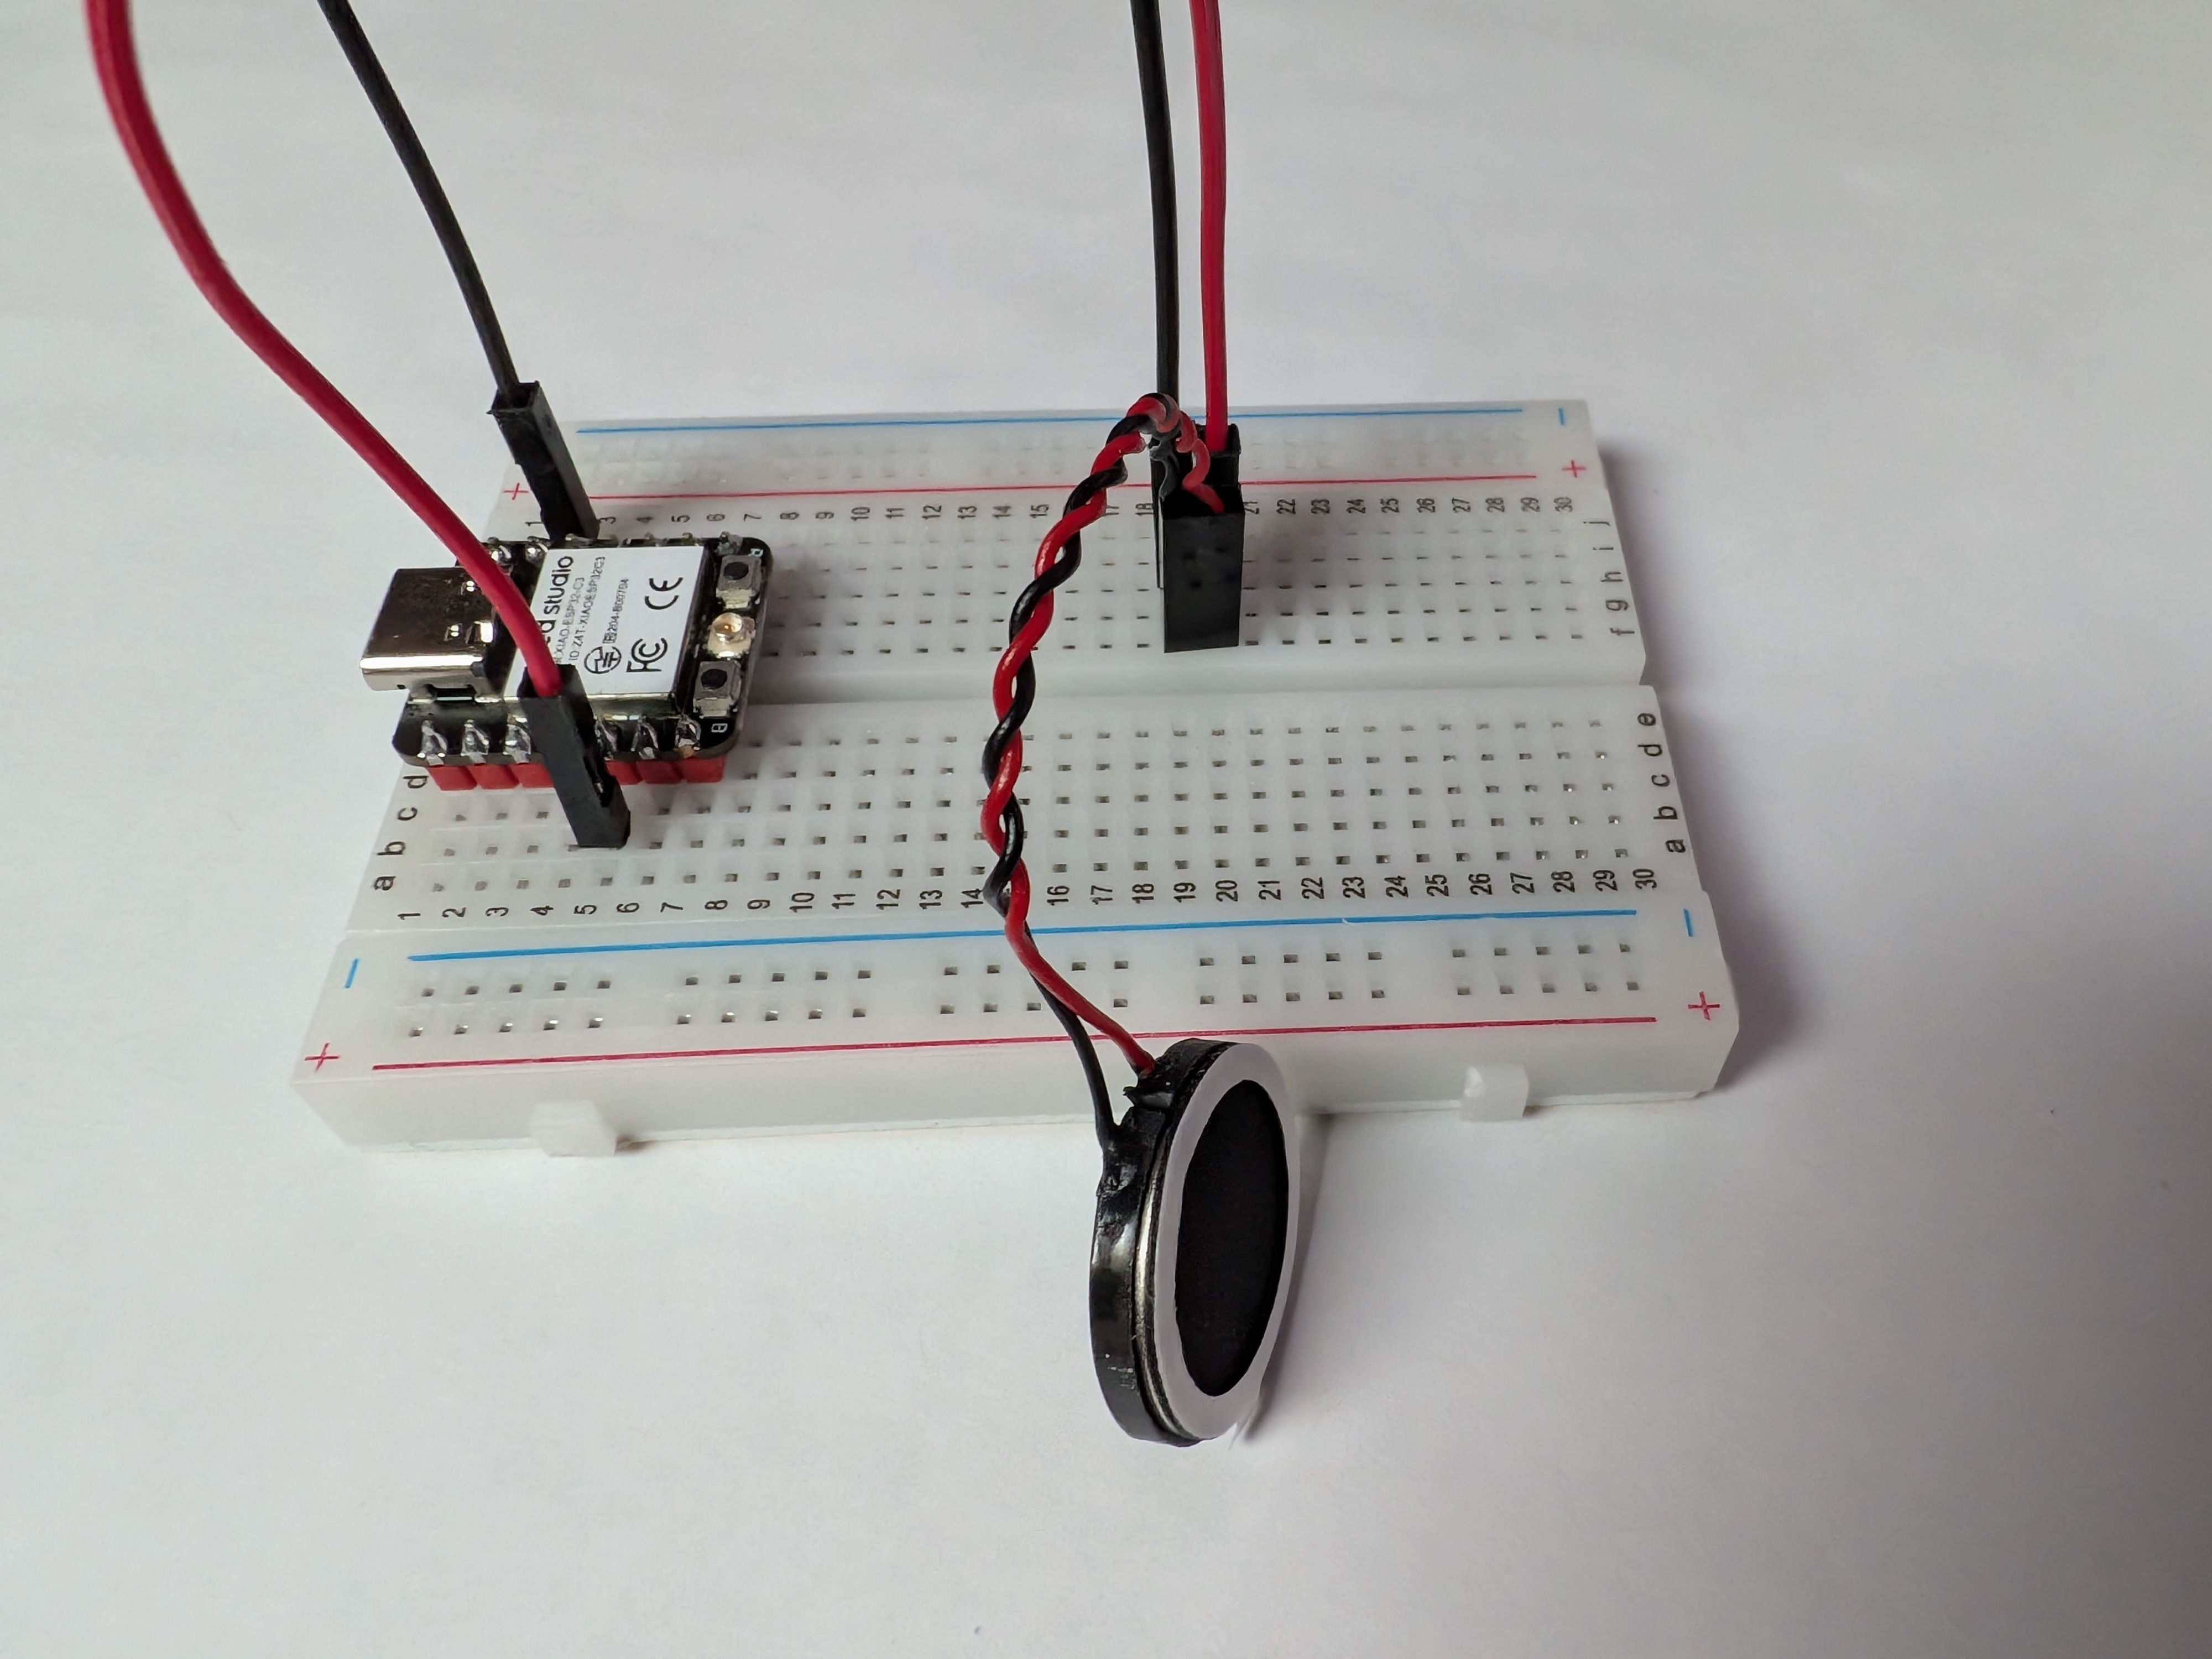
\includegraphics[width=.6\linewidth]{project_7/speaker_connected.jpg}
    \caption{The end result should look something like this}
\end{figure}

\pagebreak

\section{Directions}

\subsection{Creating the circuit}
Using jumper cables, you will be assembling a circuit between your microcontroller, your breadboard,
and the speaker included in your kit.

\subsubsection{Remove previous components}
Before beginning, remove any components from prior chapters including LEDs, buttons, and wires. You may leave the
microcontroller attached to the breadboard.

\subsubsection{Attach the microcontroller to the breadboard}
If it's not already, carefully insert the pins at the bottom of your microcontroller into the breadboard. Refer back
to \ref{pinout} for pin labels. When placing the board into the breadboard, make sure that the microcontroller is oriented such that:
\begin{itemize}
    \item The pin labeled \textbf{5V} is inserted in hole at \textbf{Column H, Row 1} of the breadboard (or \textbf{H1}, for short)
    \item The pin labeled \textbf{GPIO2} is inserted in hole \textbf{D1} of the breadboard
    \item The pin labeled \textbf{GPIO20} is inserted in hole \textbf{H7} of the breadboard
    \item the pin labeled \textbf{GPIO21} is inserted in hole \textbf{D7} of the breadboard
\end{itemize}
You may need to apply more pressure than expected to seat the microcontroller properly in the breadboard. When its over, it should look like this:
\begin{figure}[H]
    \centering
    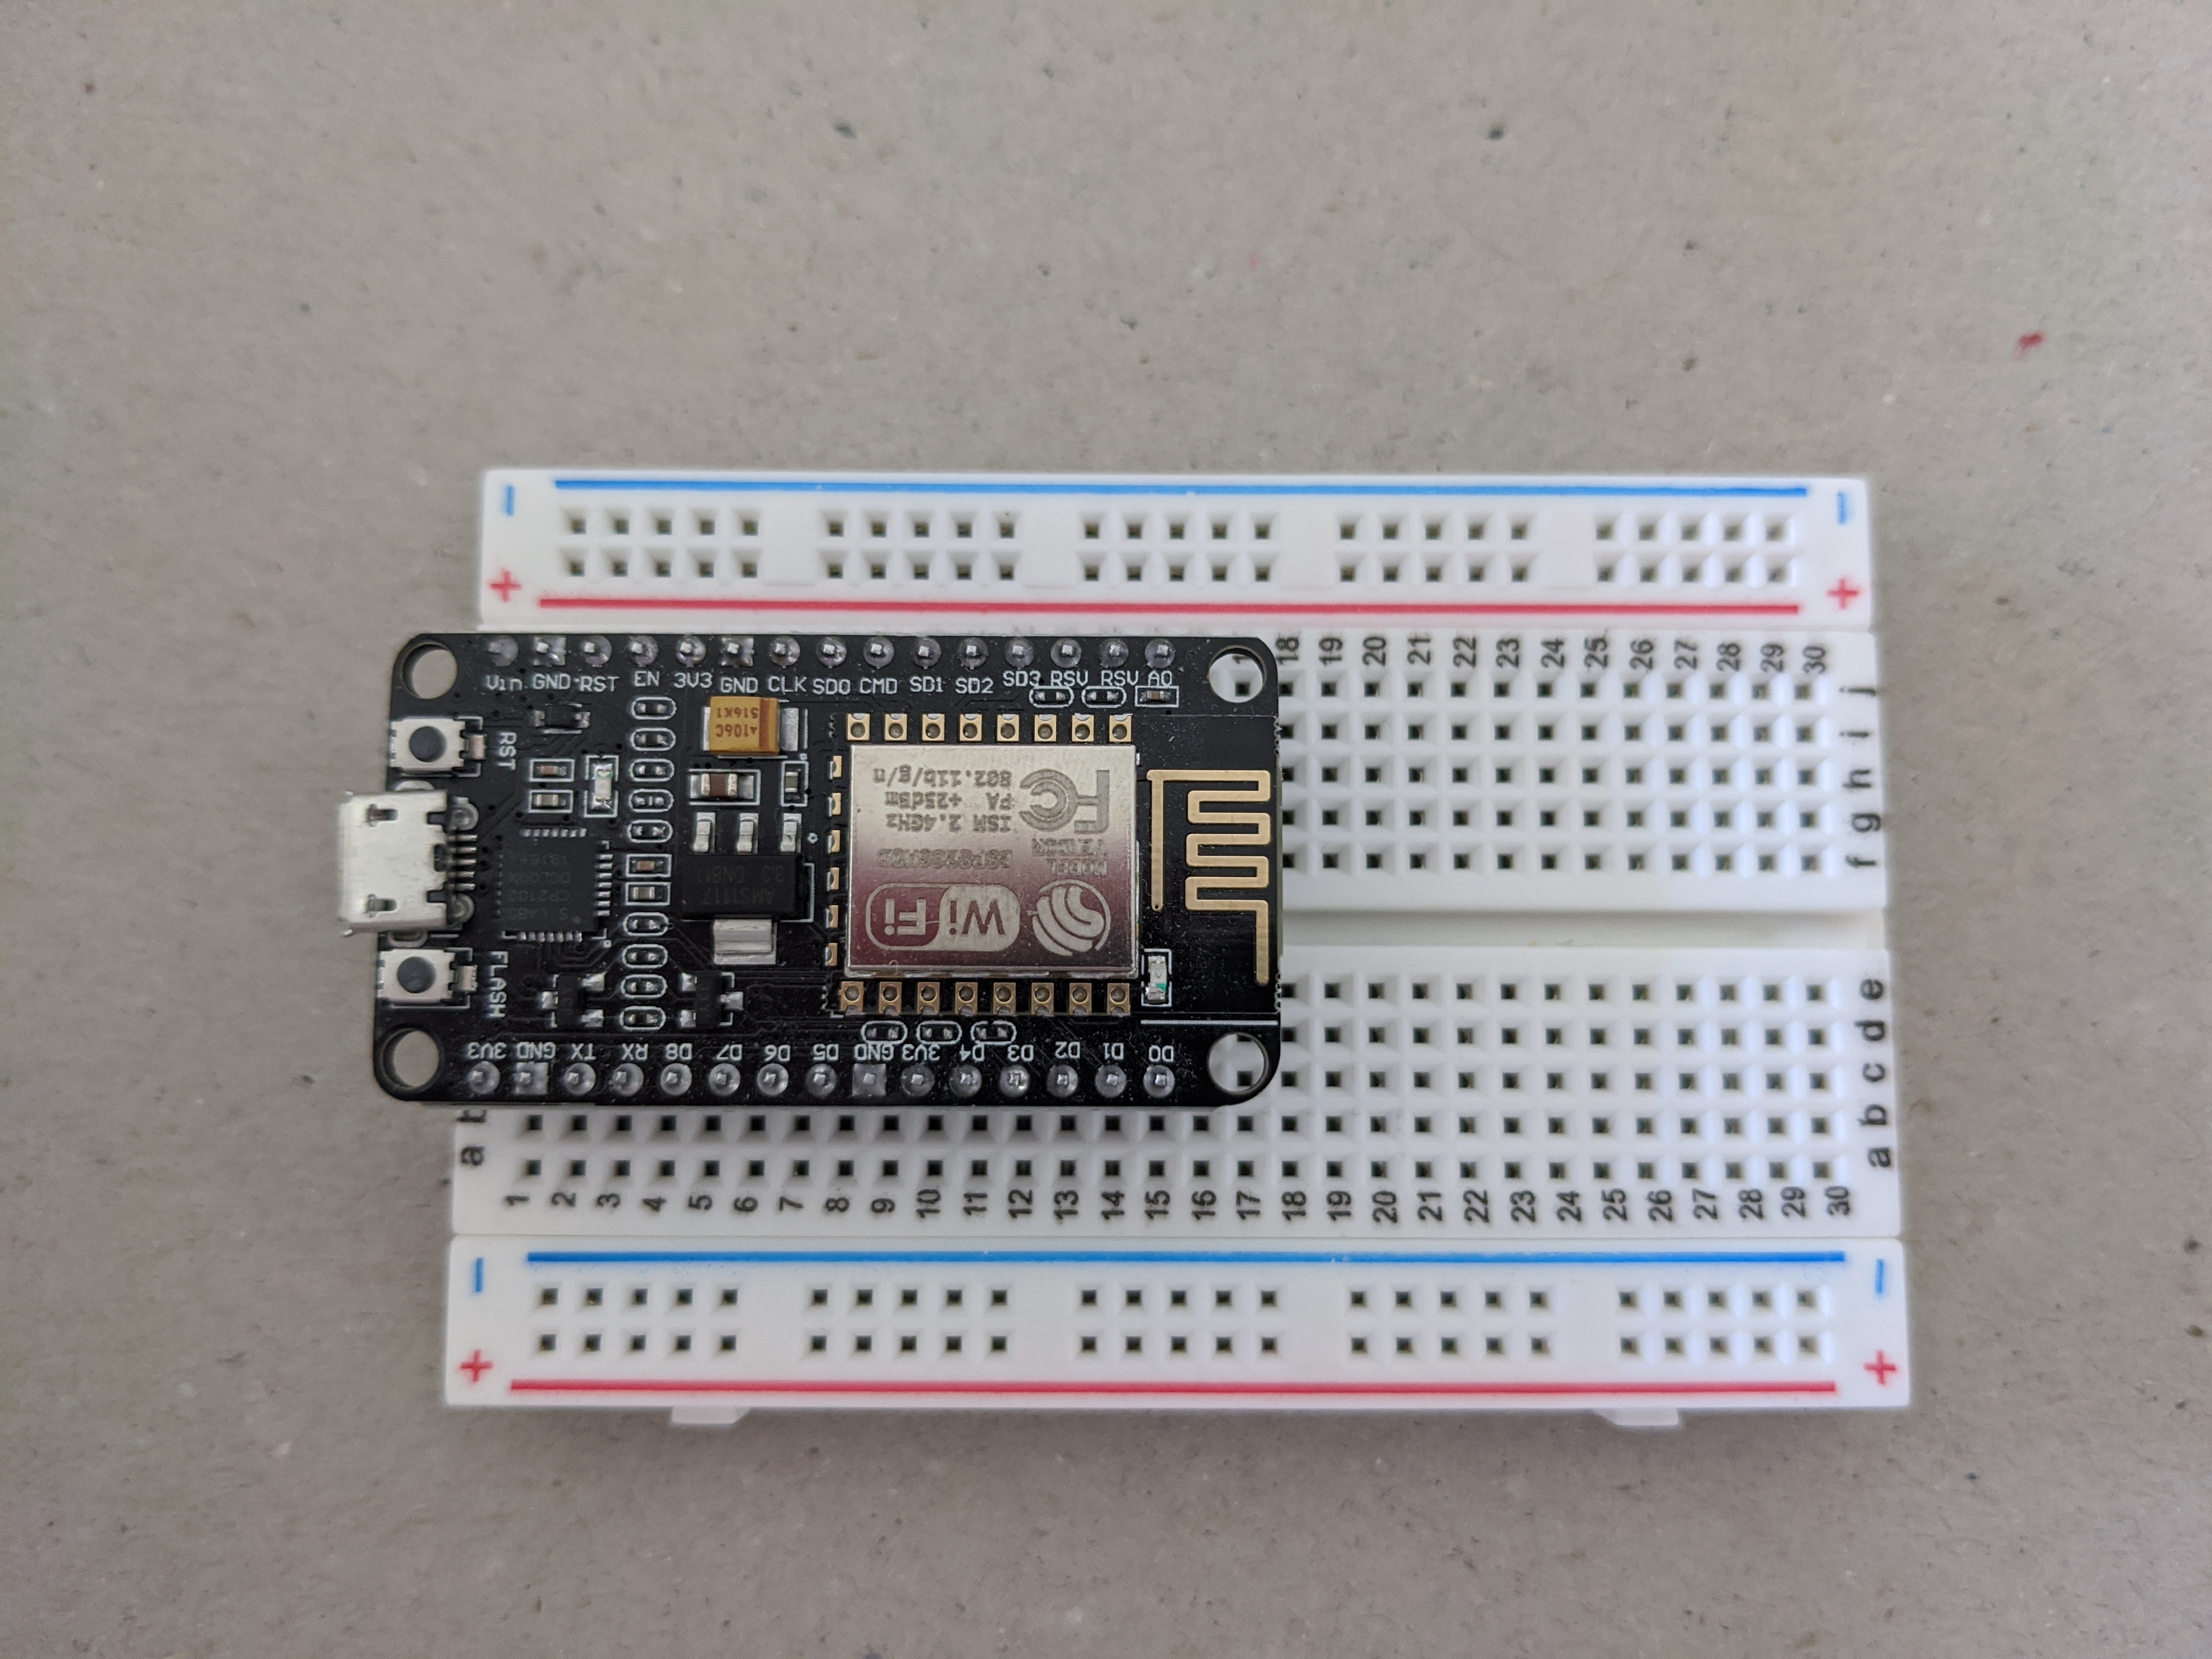
\includegraphics[width=.6\linewidth]{common/microcontroller_seated_in_breadboard.jpg}
    \caption{So far, so good!}
\end{figure}

\subsubsection{Place the Speaker on the Board}
Place the speaker into the board such that the black wire is in hole \textbf{F19}
and the red wire is in hole \textbf{F20}.

You should be left with something that looks like this:
\begin{figure}[H]
    \centering
    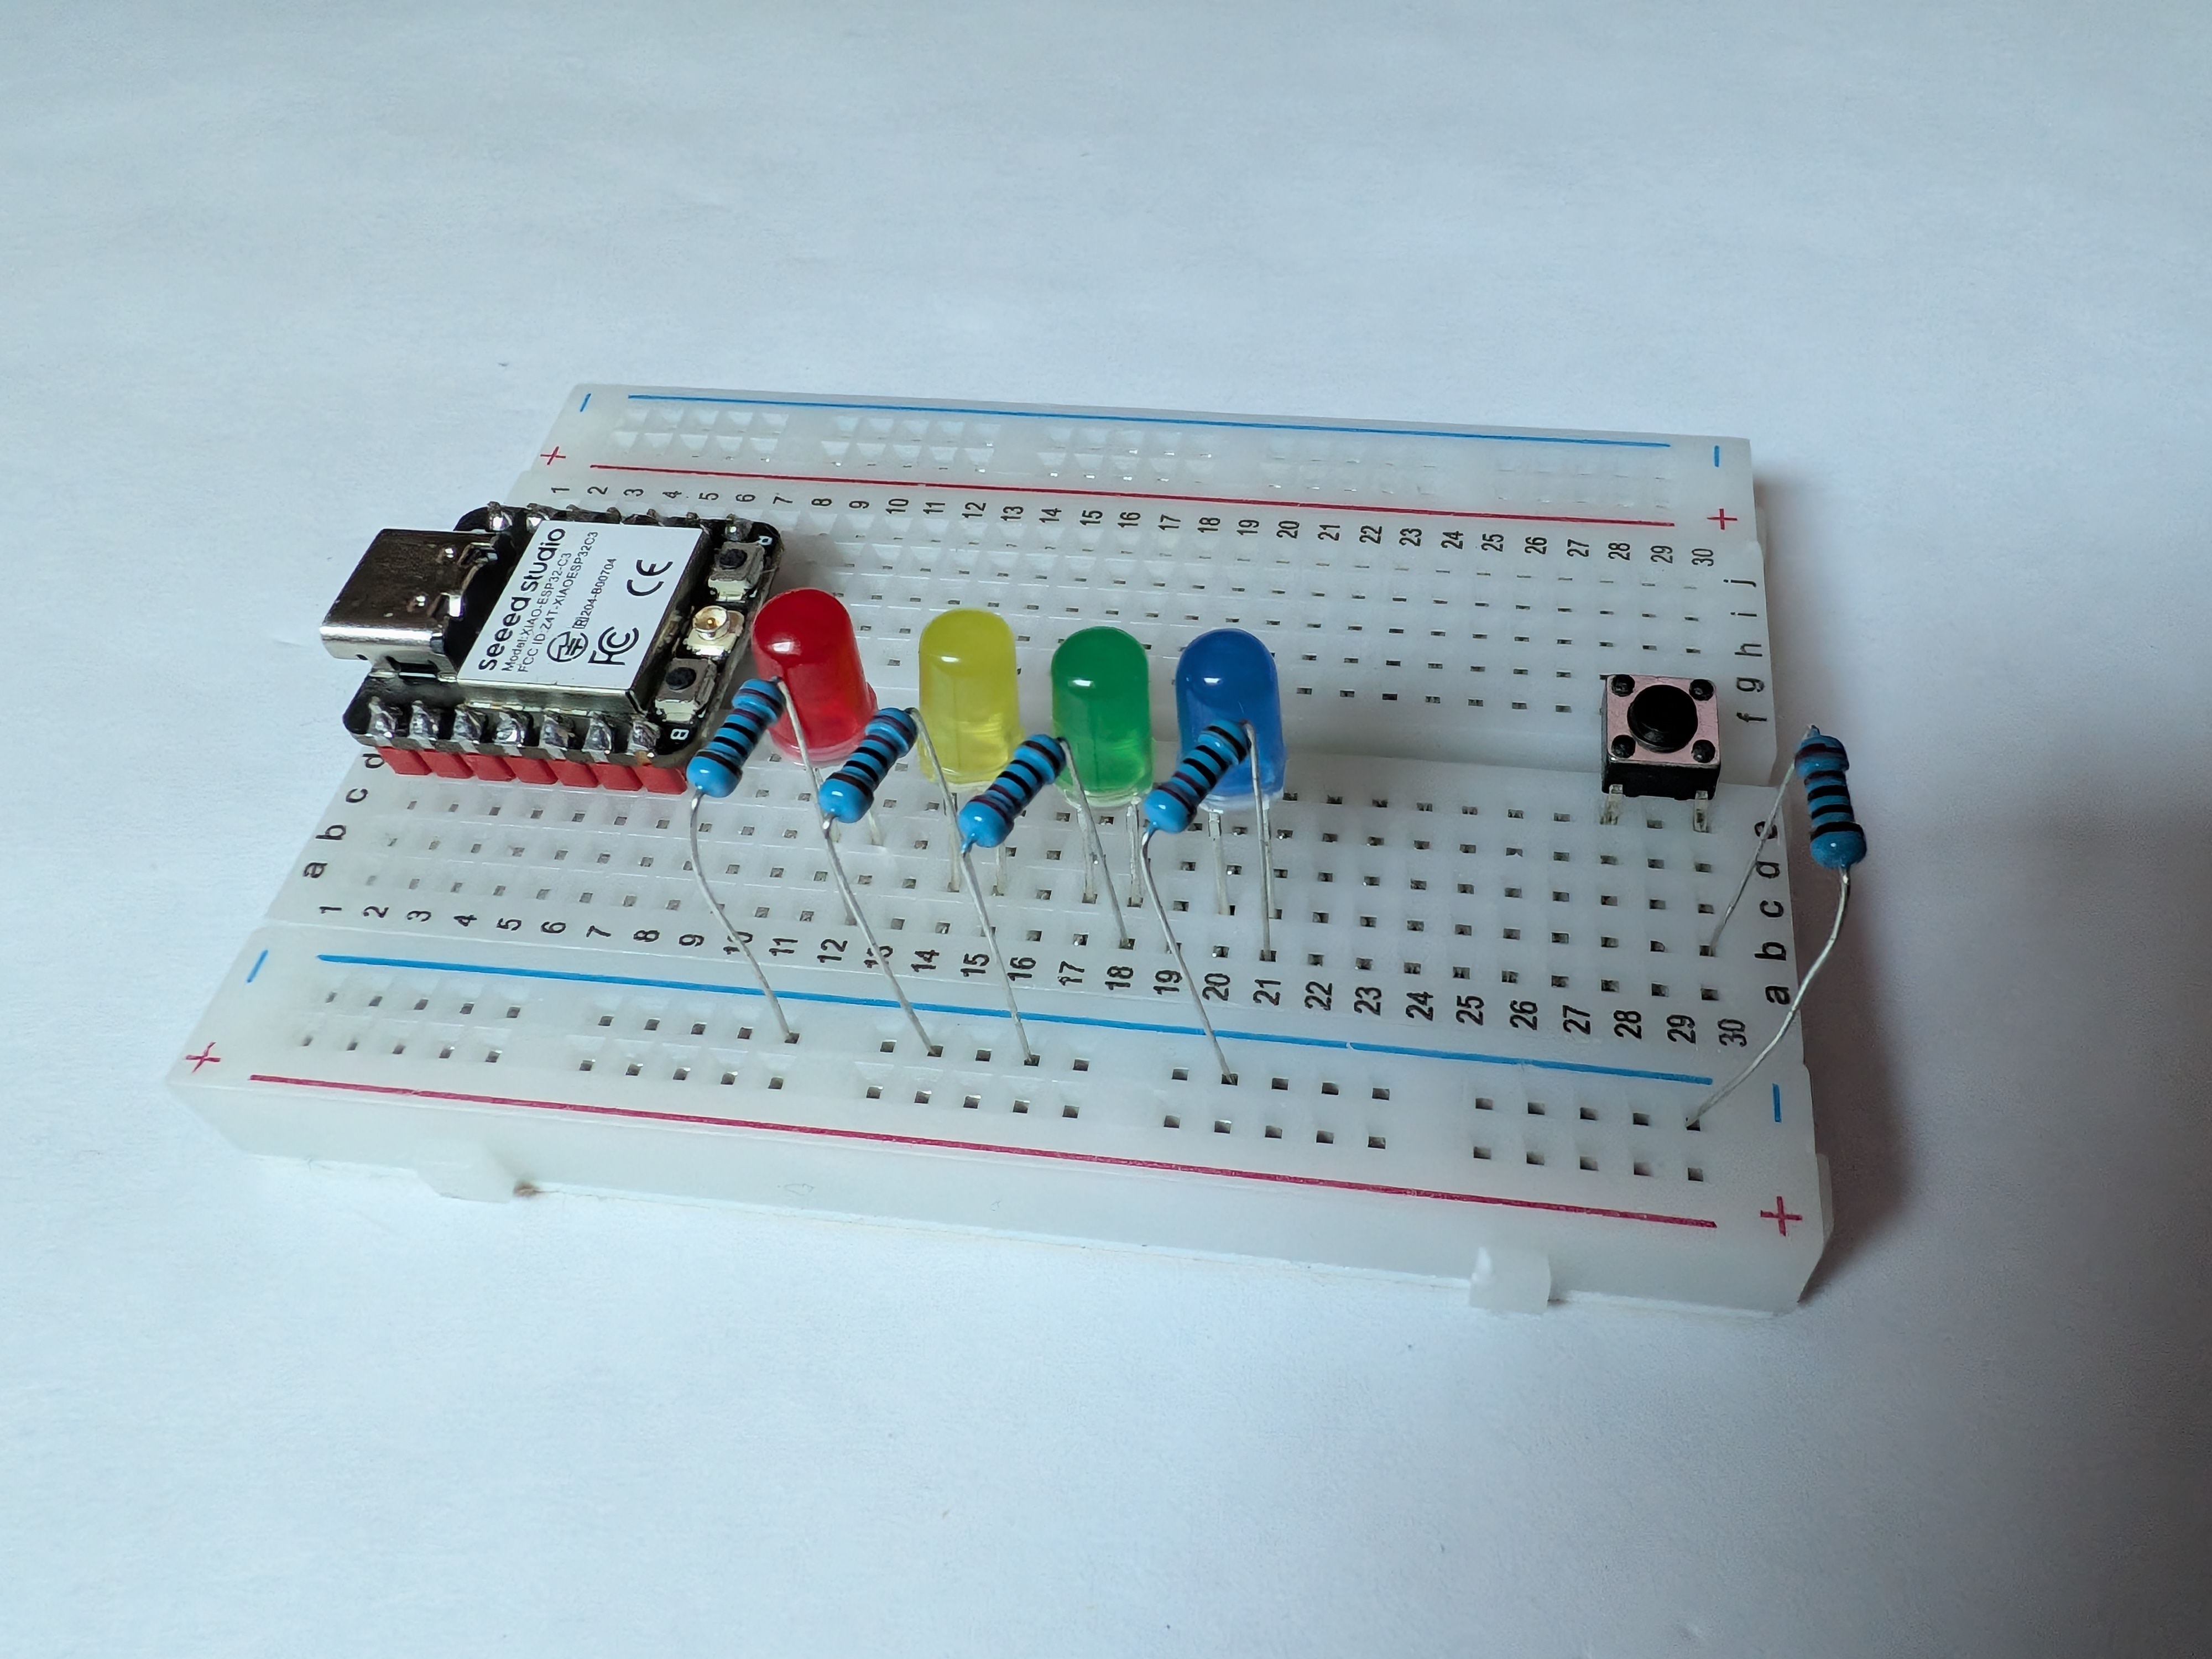
\includegraphics[width=.6\linewidth]{project_7/components_placed.jpg}
    \caption{All of the components except for the jumper wires are now placed.}
\end{figure}

\subsubsection{Connect the necessary jumper wires}
\begin{itemize}
    \item Place one end of a red jumper wire into hole \textbf{B5} of the breadboard and the other end into
    \textbf{H20}. This will provide the on/off signal to the speaker according to our program's needs.
    \item Using a black jumper wire, place one end of the wire into hole \textbf{I2} of the breadboard and the other
    end into \textbf{C12}, matching the black wire of the speaker. This will provide it's ground connection.
\end{itemize}

You should be left with something that looks like this:
\begin{figure}[H]
    \centering
    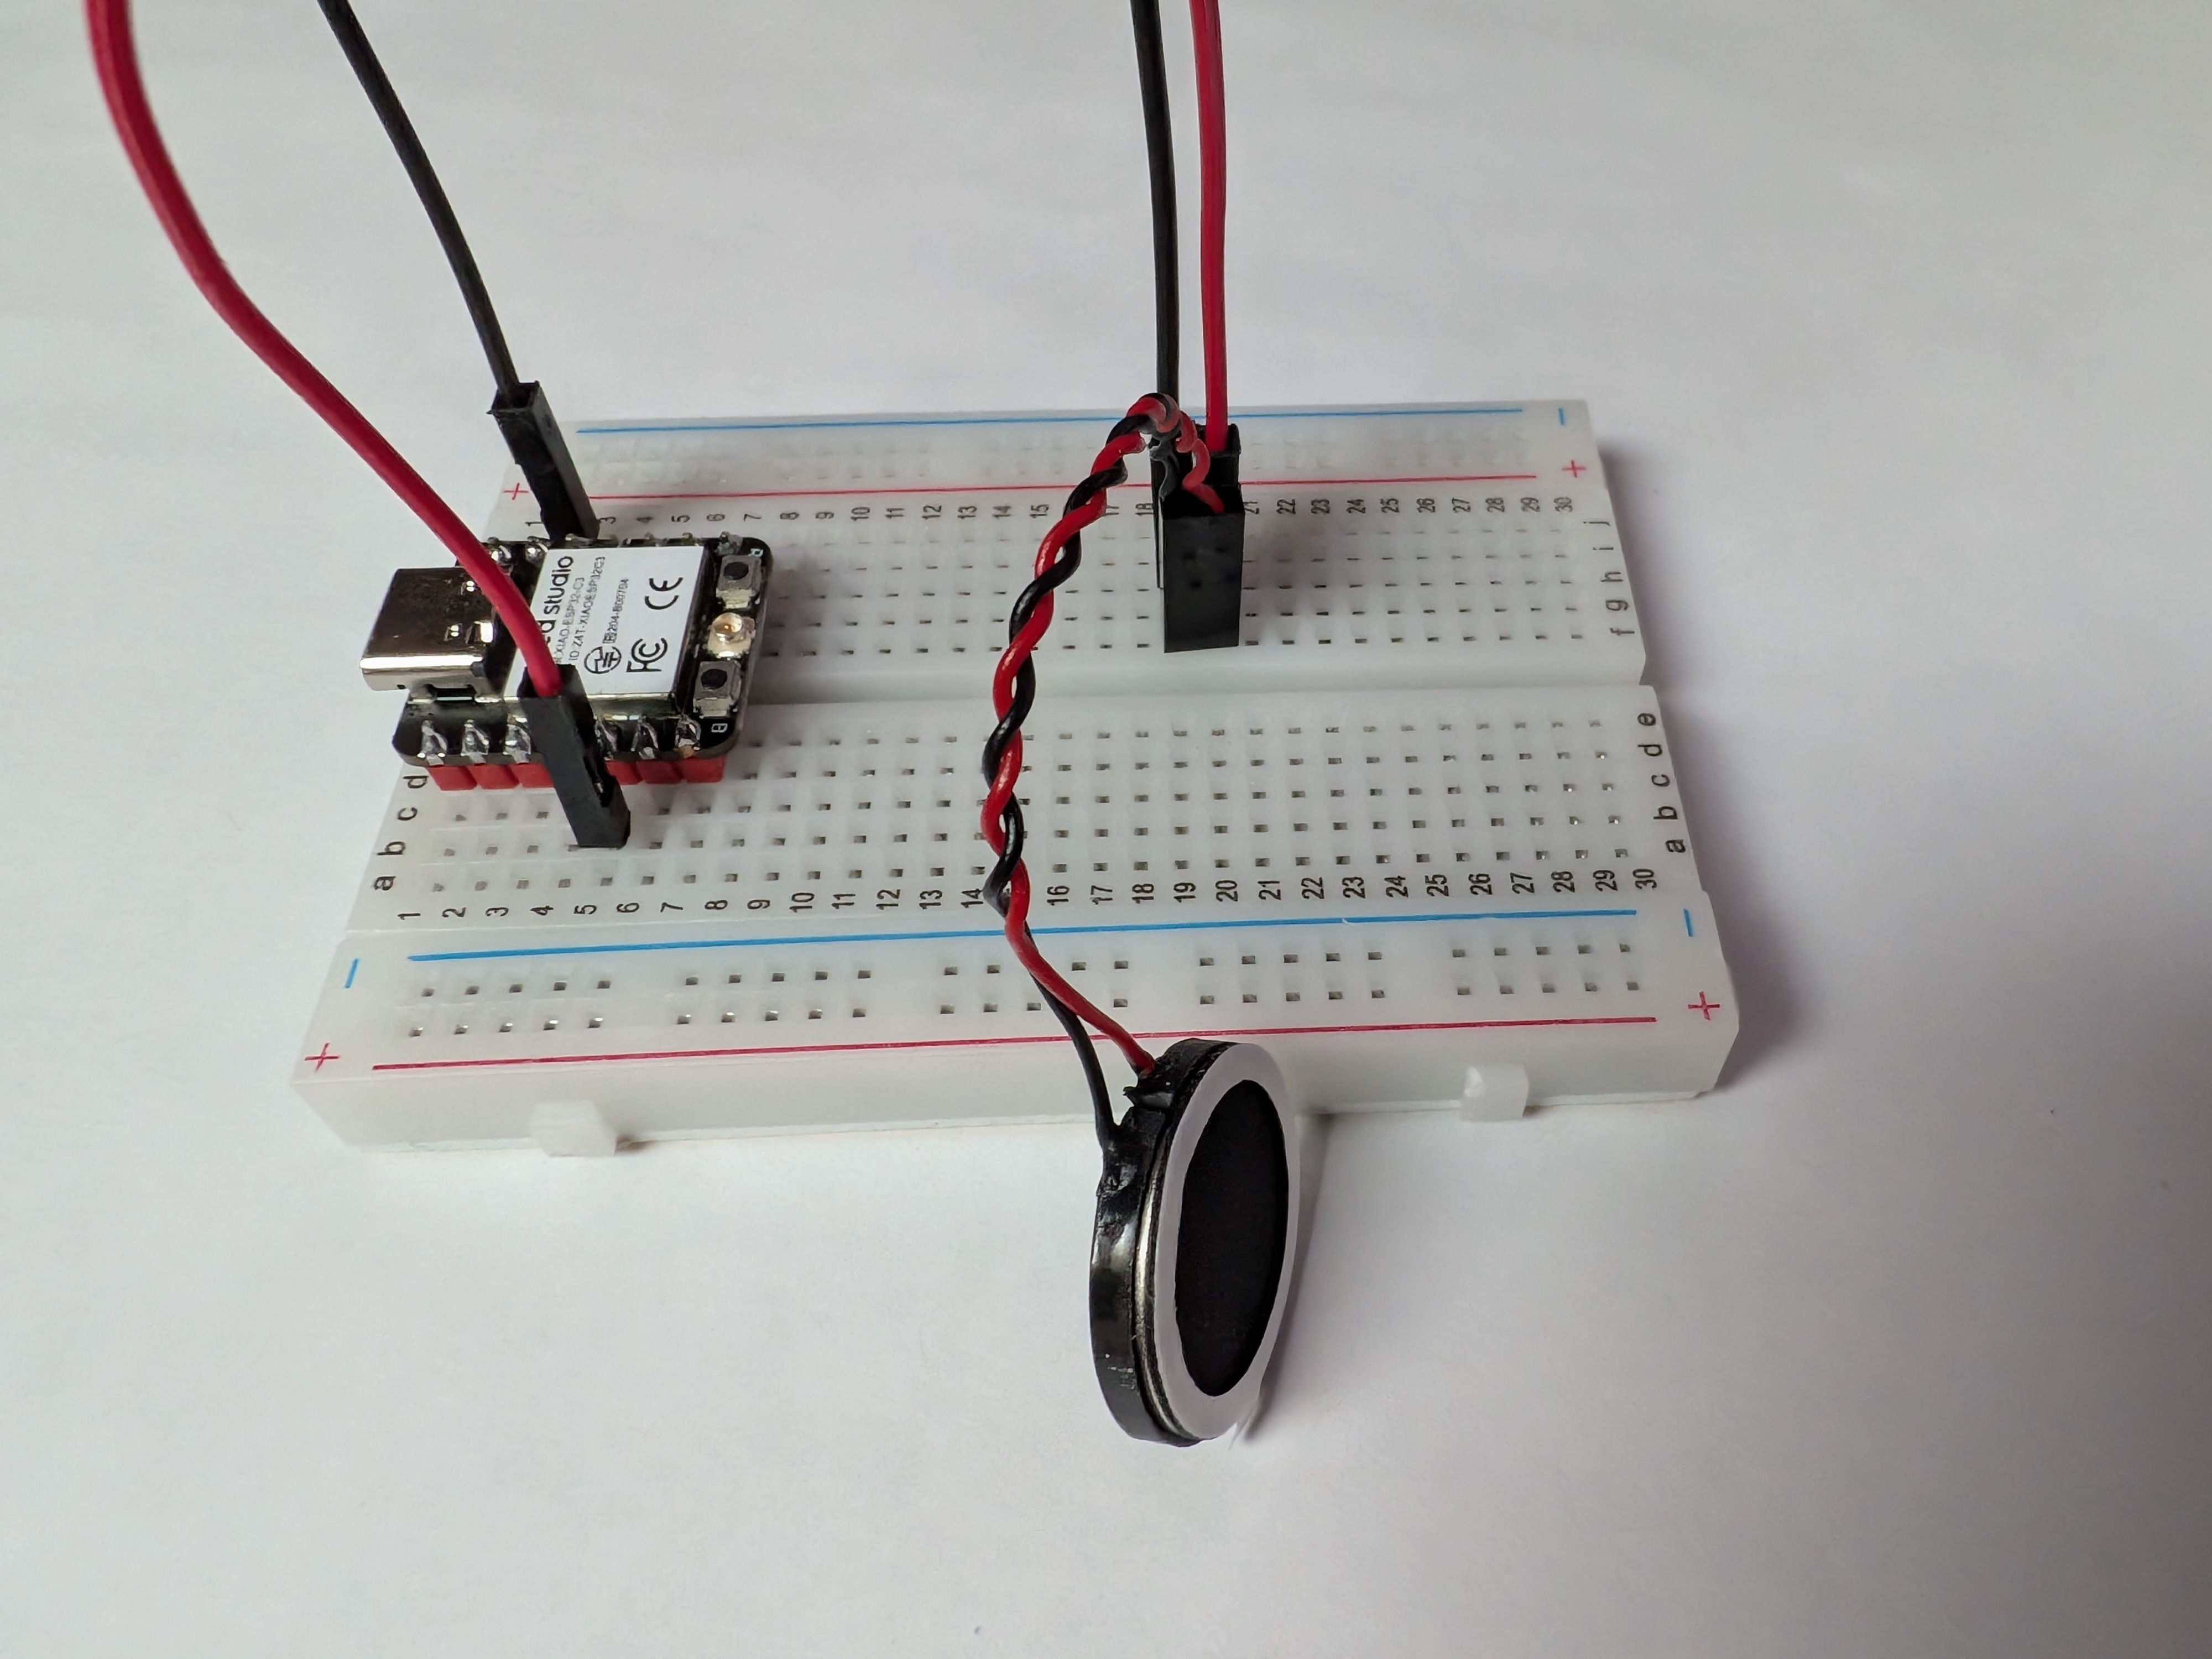
\includegraphics[width=.6\linewidth]{project_7/speaker_connected.jpg}
    \caption{All components and wires are now installed}
\end{figure}

\subsection{Programming the microcontroller}
Once all of the wiring is correct, connect the USB cable to the microcontroller (you will want to push the cable underneath the
two resistors on the left) and go to https://viper-ide.org/ in your computer's web browser. Click on the USB icon in the top
right and choose your microcontroller from the list:

\begin{figure}[H]
    \centering
    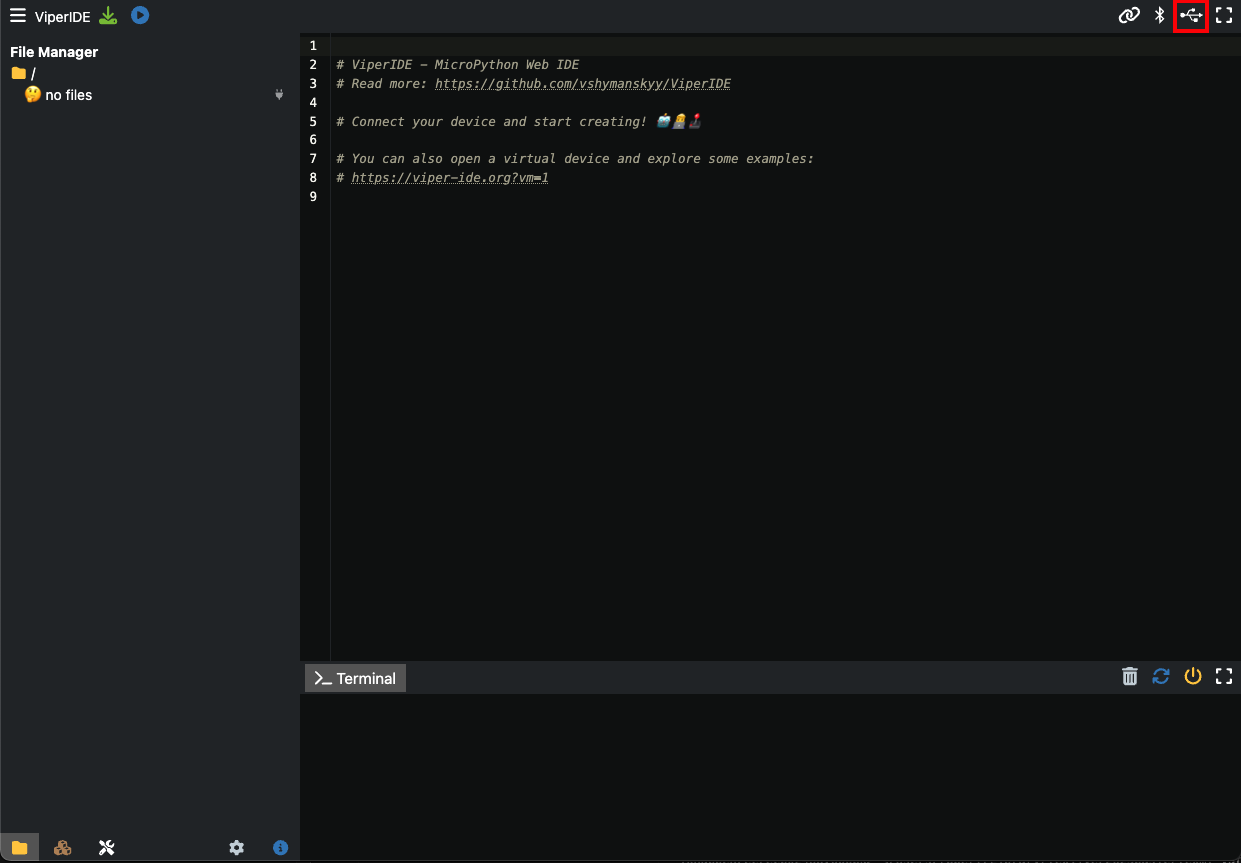
\includegraphics[width=.6\linewidth]{common/viper_ide_usb_connect.png}
    \caption{Click the button highlighted in red.}
\end{figure}

If you see multiple items in the dialog that pops up, choose the one that starts with "USB JTAG". See below for an example:
\begin{figure}[H]
    \centering
    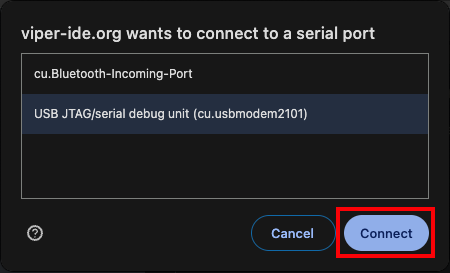
\includegraphics[width=.6\linewidth]{common/viper_ide_usb_choice_connect.png}
    \caption{Click the button highlighted in red.}
\end{figure}

Once you have connected, you will see a green dialog labeled "Device connected" and the file manager on the list
will populate with the list of files installed on the device:
\begin{figure}[H]
    \centering
    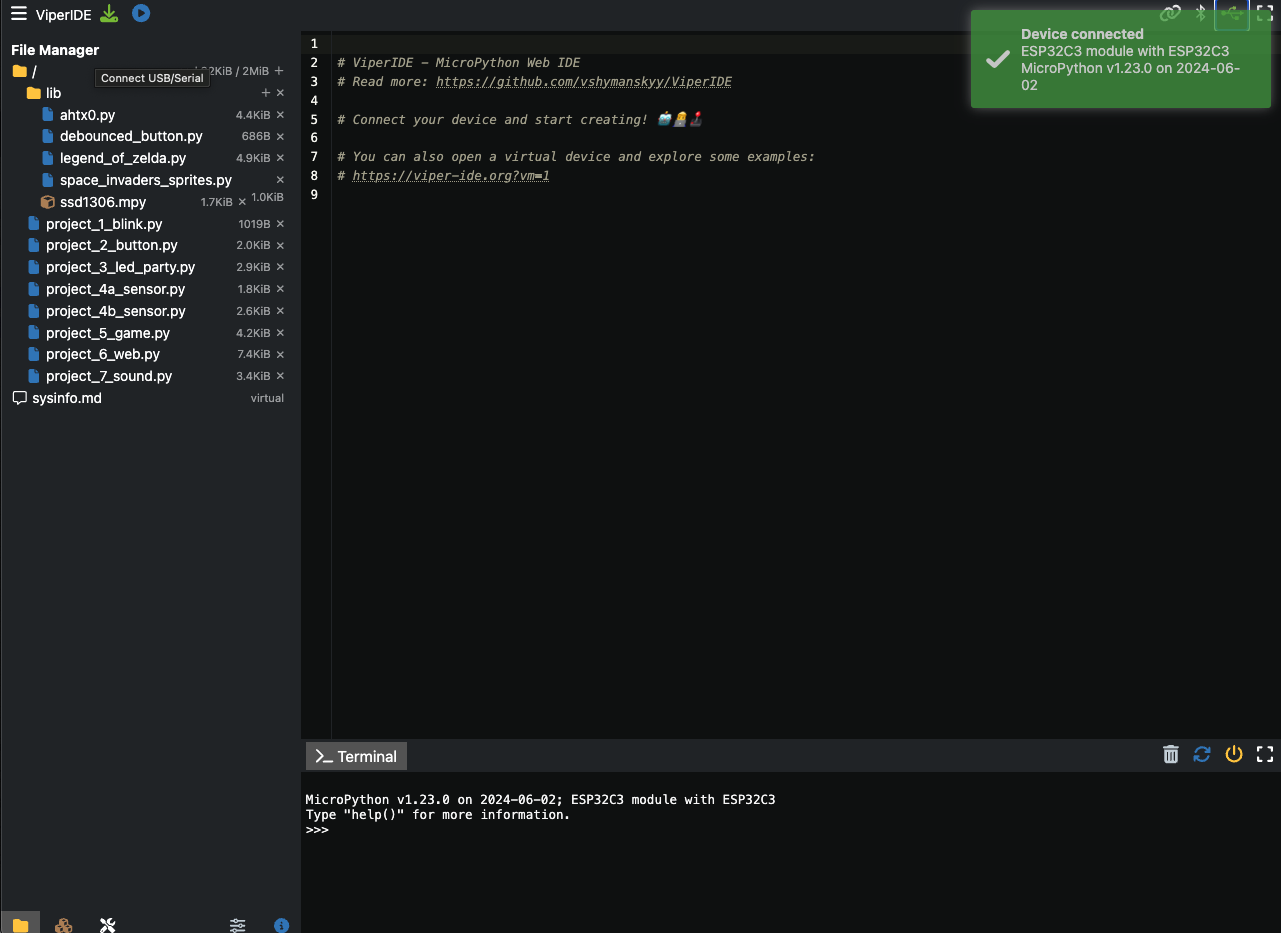
\includegraphics[width=.6\linewidth]{common/viper_connected.png}
    \caption{Make sure to open the right file for this project}
\end{figure}

Click on the file named "project\_7\_sound.py". This will load the code in the editor for this section. Read through the comments
and the code to get a sense for how it works. Once you are ready, you can click the blue play button in the upper left of the window
to start the program.

The speaker should start playing sound. See if you can recognize the tune!

\subsection{Examining the code}

This project's code shows a few new concepts:
\begin{itemize}
    \item Configuring a pin on the microcontroller as a PWM device
    \item Using \textbf{time.sleep\_ms()} calls in our code to wait a certain amount of time
\end{itemize}

Let's take each of these and examine them closer

\subsubsection{Setting up PWM}
\begin{lstlisting}[language=Python,caption=PWM Mode]
    # set the notes and sleep for the appropriate time
    pwms = [PWM(pin, freq=note, duty=instrument) for pin in pins]
\end{lstlisting}

PWM stands for Pulse Width Modulation. When we configure the PWM object by passing
a pin object, it instructs the microcontroller to start pulsing that pin at the given
frequency and duty cycle. By pulsing, we mean that the voltage on the pin goes up and
down at a fixed rate. If you've heard that humans can hear frequencies between 20Hz and 20,000Hz,
this is an example of that same thing. In this case, we are going to pulse the pin at
a certain frequency based on the note we want to hear.

The code has a list of notes and the associated frequencies in it. Here's a snippet:

\begin{lstlisting}[language=Python,caption=Note names mapped to frequencies]
    ("G#0", 208),
    ("A1", 220),
    ("Bb1", 233),
    ("B1", 247),
    ("C1", 262), # middle C
    ("C#1", 277),
    ("D1", 294),
\end{lstlisting}

From this list, we can see that middle C (that is, the note named C that is in the middle
of a full sized piano) is associated with a frequency of 262Hz. Or in other words, if we
want to hear a middle C out of our speaker, then we need to pulse the pin on and off 262
times per second.

The other important argument is releated to the duty cycle. Duty cycle means the amount
of time the pin is on vs. the amount of time the pin is off. For example, a 50\% duty cycle
is when the pin is on for half of the time and off for half of the time. A 75\% duty cycle
is when the pin is on for 3/4 of the time and off for 1/4 of the time. Here's what that
would look like visually:

\begin{figure}[H]
    \centering
    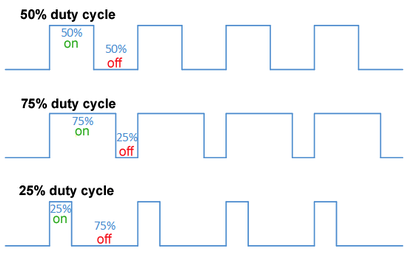
\includegraphics[width=.6\linewidth]{project_7/duty_cycle.png}
    \caption{Examples of 3 different duty cycle settings}
\end{figure}

You can play with the duty cycle to make the resulting notes sound like different instruments.
In the code, this is done with this mapping:

\begin{lstlisting}[language=Python,caption=Instrument names mapped to duty cycle settings]
INSTRUMENTS = {
    "trumpet": 64,
    "clarinet": 512,
    "keyboard": 700,
}
\end{lstlisting}

The numbers here represent the number of milliseconds (out of 1000 milliseconds in 1 second)
that the pin should be on. The instrument names give some idea about how it might sound, but
these are only very rough approximations!

\subsubsection{Going to sleep}

Another important part of music (and some might say the most important part) is resting.
A rest in music is a period of time when no note is being played. In order to implement
this in our code, we call the \textbf{time.sleep\_ms()} function and then return without
setting any of the pins to pulse. The \textbf{time.sleep\_ms()} tells the microcontroller to
do nothing for the given amount of time before it moves to the next line of code.

\begin{lstlisting}[language=Python,caption=Using the sleep function]
    # if this is a rest, then just sleep
    if not note:
        time.sleep_ms(duration)
        return
\end{lstlisting}


\section{Review}

In this project, you saw how a microcontroller plus some code can be used to make
a speaker make sounds. While this project only makes simple types of sounds, you
can get much fancier with some additional code and hardware and play .mp3 files
from an attached SD card or even stream web-based radio stations!

\section{Possible Extensions}
If you want to do some experimentation, try these:

\begin{itemize}
    \item Try playing with the duty cycle to see if you can come up with other instrument sounds
    \item Try creating your own songs by using the same format as the example song
\end{itemize}
